\documentclass{article}

\usepackage{fancyhdr} % Required for custom headers
\usepackage[utf8]{inputenc}
\usepackage{lastpage} % Required to determine the last page for the footer
\usepackage{extramarks} % Required for headers and footers
\usepackage[usenames,dvipsnames]{color} % Required for custom colors
\usepackage{graphicx} % Required to insert images
\usepackage{listings} % Required for insertion of code
\usepackage{color, xcolor}
\usepackage{courier} % Required for the courier font
\usepackage{lipsum} % Used for inserting dummy 'Lorem ipsum' text into the template
\usepackage[norsk]{babel}
\usepackage{amsmath}

% Margins
\topmargin=-0.45in
\evensidemargin=0in
\oddsidemargin=0in
\textwidth=6.5in
\textheight=9.0in
\headsep=0.25in

\linespread{1.1} % Line spacing

% Set up the header and footer
\pagestyle{fancy}

\lhead{\exerciseGroup} % Top left header
\chead{\exerciseClass: \exerciseTitle} % Top center head
\rhead{\firstxmark} % Top right header
\lfoot{\lastxmark} % Bottom left footer
\cfoot{} % Bottom center footer
\rfoot{Page\ \thepage\ of\ \protect\pageref{LastPage}} % Bottom right footer
\renewcommand\headrulewidth{0.4pt} % Size of the header rule
\renewcommand\footrulewidth{0.4pt} % Size of the footer rule

\setlength\parindent{0pt} % Removes all indentation from paragraphs


% Document data

\newcommand{\exerciseTitle}{Øving 6} % Assignment title
\newcommand{\exerciseClass}{TMA4280} % Course/class
\newcommand{\exerciseGroupMembers}{Sindre Magnussen og Håkon Åmdal}
%----------------------------------------------------------------------------------------
%	TITLE PAGE
%----------------------------------------------------------------------------------------
\newcommand{\HRule}{\rule{\linewidth}{0.5mm}}
\title{
\vspace*{\stretch{1}}
\noindent\HRule
\begin{center}
 \Huge
 \noindent	\exerciseClass \\
 \noindent \exerciseTitle \\ [4mm]
 \large
 \noindent\emph{\exerciseGroupMembers}
\noindent\HRule \newline
\end{center}
\vspace{0cm}
\begin{center}
	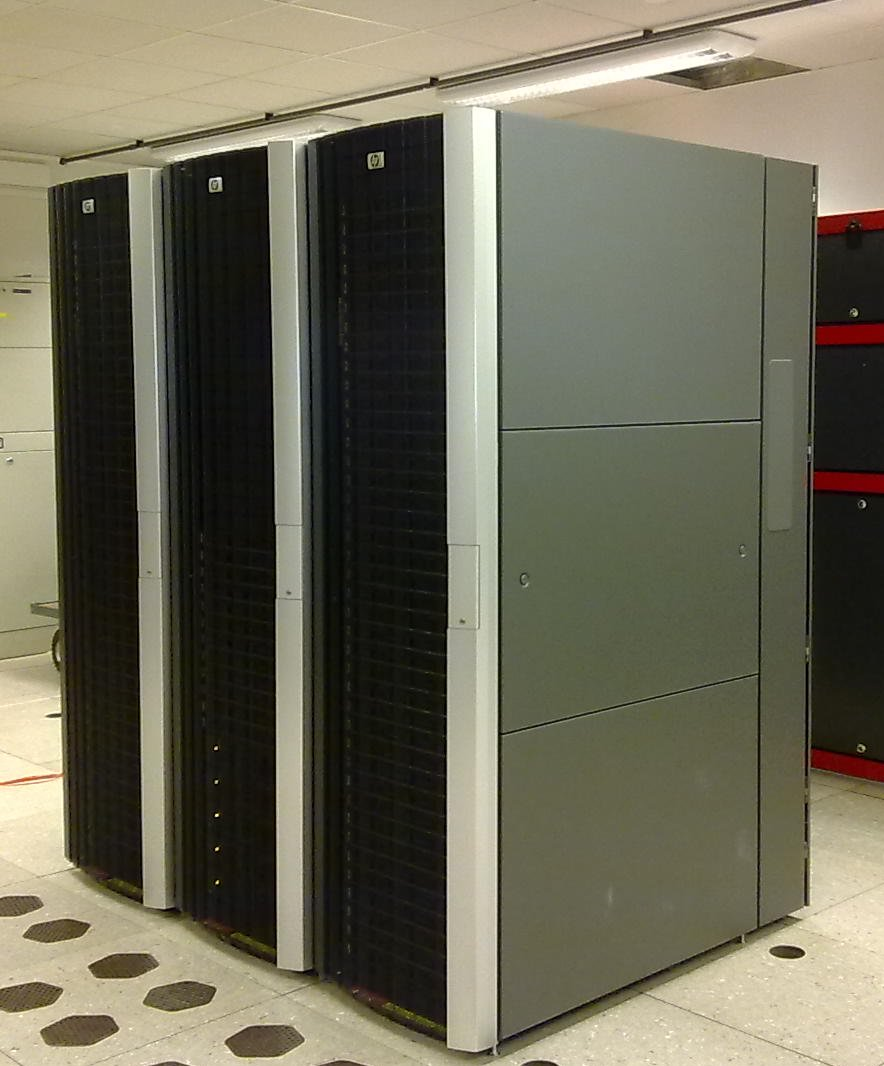
\includegraphics[width=10cm]{img/kongull.jpg}
\end{center}
\vspace*{\stretch{3}}
\begin{center}
\end{center}
}
% Insert date here if you want it to appear below your name

\newcommand{\ub}[1]{\underbar{$#1$}\,}
\definecolor{mygreen}{rgb}{0,0.6,0}
\definecolor{mygray}{rgb}{0.5,0.5,0.5}
\definecolor{mymauve}{rgb}{0.58,0,0.82}
\lstdefinestyle{customc}{
  belowcaptionskip=1\baselineskip,
  breaklines=true,
  frame=L,
  xleftmargin=\parindent,
  language=C,
  showstringspaces=false,
  basicstyle=\footnotesize\ttfamily,
  keywordstyle=\bfseries\color{green!40!black},
  commentstyle=\itshape\color{purple!40!black},
  identifierstyle=\color{blue},
  stringstyle=\color{orange},
}
\lstset{escapechar=@,style=customc}


\begin{document}
\pagestyle{empty}
\maketitle

\thispagestyle{empty}

\newpage \tableofcontents


\newpage

\pagenumbering{arabic}

\section{Introduksjon - Poisson-problemet}
Poisson-ligningen er en av de mest kjente partielle diffensialligingene, og skrives på formen:
\begin{equation}
	-\nabla^2 u = f
\end{equation}
Her er $\nabla^2$ kjent som Laplace-operatoren.\\
\\
Liginingen brukes som en matematisk modell til å beskrive flere fysiske systemer, som oftest diffusjonsprosesser. Eksempler på typiske fysiske fenomener hvor poisson-ligningen kan brukes som modell er beregning av elektrisk felt, tilnærminger av strømninger i fluider og varmeoverføring uten varmetap. Poisson-ligingen dukker også opp når man skal regne ut egenverdier.\\
\\
Et poissonproblem er et problem der man skal finne en løsning til poisson-ligningen gitt en funksjon $f$ og et domene. Domenet har også grensebetingelser, slik at problemet har en unik løsning. Problemet vi skal løse i denne øvingen lyder som følgende:
% Dette er tatt direkte fra ps6.tex %
\begin{eqnarray}
	-\nabla^2 u & = & f \hspace{.5in} \textrm{in} \,\,\, \Omega = (0,1)\times (0,1) \\
	u & = & 0 \hspace{.5in} \textrm{on} \,\,\, \partial\Omega\, .
\end{eqnarray}
Her er $f$ en funksjon vi kjenner,  og $u$ er løsningen vi skal komme frem til. Vi har gitt at et enhetskvadrat  er vårt domenee, og at verdiene i kantene av dette kvadratet er $0$ (homogene Dirichlet grensebetingelser). En annen forutsetning er at $f$ må ligge i L2.\\
\\
Siden denne skal løses på en datamaskin, og en datamaskin har begrenset med ressurser (minne/regnekraft), må vi finne en tilnærming til løsningen $u$. Det finnes flere måter å diskretisere poisson-ligningen på, blant annet endelige differanser, endelige elementer og endelige volumer. Felles for disse er at alle ender opp med et sett med ligninger som kan skrives på formen:
\begin{equation}
	\label{eq:linear-system}
  \ub{A} \ub{u} = \ub{g}
\end{equation}

\begin{figure}[t]
	\label{fig:finite-difference}
	\centering
	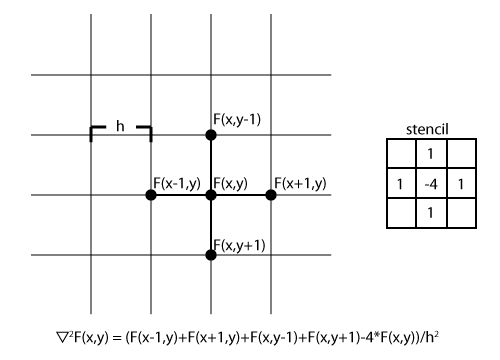
\includegraphics[width=10cm]{img/finite-difference.png}	
	\caption{Oppretting av et ligningsystem ved hjelp av endelige differanser. Figur funnet i \cite{rdw}. }
	
\end{figure}

Siden \emph{TMA4280} underviser i endelige differanser, og dette er ofte beskrevet som den enkleste metoden, er dette også utgangspunktet for denne oppgaven. Oppgaven beskriver et todimensjonalt poissonproblem, og da fylles ligningssettet ut med en maske som vist i figur \ref{fig:finite-difference} (fempunktsformelen).

\section{Mulige løsningsstragegier}
Når vi har fått et ligningssystem på formen vist i ligning \ref{eq:linear-system}, gjenstår det å finne en metode å løse dette på. Det finnes mange metoder, og noen av metodene utnytter egenskaper ved ligningssystemene fra poissonproblemet for å effektivisere plassforbruk og kjøretid.
\subsection{Direkte metoder}
Dirkete metoder løser et system med ligninger i et endelig og forutsigbart antall steg, og er spesielt egnet når matrisene er symmetriske og positivt definitt (som ligningssettet produsert ved hjelp av endelige differanser). Eksempelet på den mest generiske direkte metoden er LU-faktorisering, med følgende asymptotiske egenskaper:
\begin{align*}
      \mathcal{N}_{op} &\sim \mathcal{O}(N^3), \\
      \mathcal{M} &\sim \mathcal{O}(N^2).
\end{align*}
Her er $N$ antall ukjente,  $\mathcal{N}_{op}$ antall FLOP og $\mathcal{M}$ minnebruk (i bytes). Flere optimaliseringer av LU-faktoriseringer finnes, det er særlig vanlig å utnytte at matrisen er glissen for å redusere minnebruk og antall flyttallsoperasjoner. \\
\\
Ved å utnytte ligningen som blir generert av fem-punktsformelen, kan vi diagonalisere ligningssystemet ved hjelp av egenvektorer og egenverdier, siden disse da er lette å regne ut. Grunnen til dette er at ligningssystemet vårt kan representeres ved et tensorprodukt.\\
\\
En av disse diagonaliseringsmetodene benytter seg av FFT (The Fast Fourier Transform), og har følgende asymptotiske egenskaper:
\begin{align*}
  \mathcal{N}_{op} &\sim \mathcal{O}(N \log N), \\
  \mathcal{M} &\sim \mathcal{O}(N).
\end{align*}
Denne tilnærmet optimale løsningen er strategien vi skal bruke for å løse poisson-problemet i denne øvingen. FFT har et konstant minnebruk og et arbeid på $\log N$ per frihetsgrad, hvilket er veldig bra.

\subsection{Iterative metoder}
I tillegg til direkte metoder, har vi også iterative metoder. En slik metode vil oppdatere løsningen i iterasjoner, og vil (forhåpentligvis) komme nærmere og nærmere for hver gang. Iterative metoder har som oftest et uforutsigbart antall iterasjoner, og vil vanligvis måtte bli stoppet av et kriterium gitt av brukeren. Jo strengere kriterium, jo flere iterasjoner. Antall iterasjoner vil også kunne variere fra problem til problem, selv om man benytter seg av samme algoritme.\\
\\
Generelt sett, drar iterative metoder fordel av at vi ikke lenger har noen krav om hvordan matrisen er lagret, og at minnebruk ofte er proposjonalt med antall ukjente. I tillegg, består metodene ofte av grunnleggende matrise-vektor-operasjoner, som ofte er optimalisert i soft- og hardware. Til slutt, er flere av disse metodene godt egnet for parallell prossesering. \\
\\
Eksempler på iterative metoder er \emph{Gauss-Jacobi}, \emph{Gauss-Seidel}, \emph{Generalized minimum residuial method} og \emph{Conjugate gradient method}. Brukt riktig, kan disse metodene være svært kraftige.

\section{Programkomponenter}
\label{section:programkomponenter}
Rent overordnet har vi valgt å skrive nesten all kode i et felles bibliotek, og koblet på flere små programmer med ulike bruksområder. Det blir ingen nøye gjennomgang av koden i denne rapporten, da det befinner seg mange gode og beskrivende kommentarer der. Flere av funksjonene implementert regnes også som kjent av leseren av dette dokumentet, siden de er beskrevet i \cite{fast-poisson}. Det anbefales også å ta en titt på testene (beskrevet i seksjon \ref{subsection:unittest} og \ref{subsection:mpi_unittest}) for å få en dypere forståelse for input og forventet output.

\paragraph{Testing}
Vi bestemte oss tidlig for at det var langt viktigere med et program som gav riktig resultat enn et program som kjørte raskt. Vi har derfor hatt stor vekt på både enhets-testing og korrekthetstesting av løsning (konvergenstest) under utviklingen. Når programmet var ferdig, hadde vi derfor tilstrekkelig testdekning til å gjøre optimaliseringer. Bruk av tester har også forenklet kommunikasjonen mellom gruppens to medlemmer.

\paragraph{Tilstand}
Alle funksjoner i \emph{ps6\_common\_library} er bevisst programmert uten tilstand, og dette fører ofte til at parameterlistene er ganske lange. Dette er kun for å forenkle enhetstestene våre. Vi er ikke kjent med overhead knyttet til parameterpassing kontra globalt definerte variabler, men vi antar at det er neglisjerbart.

\paragraph{Flagg for MPI og OpenMP}
Vi har dessverre ikke hatt fokus på å utvikle løsningen vår til å la seg kompilere uten OpenMP og/eller uten MPI. Preprosessorflaggene \emph{HAVE\_MPI} og \emph{HAVE\_OPENMP} blir brukt i noen sammenhenger, men er ikke konsekvente nok til å støtte at programmene kompileres uten at disse er på. For å kjøre programmet uten støtte for MPI har vi ikke benyttet oss av kommandoen \emph{mpirun} og for å kjøre programmet uten OpenMP har vi satt environmentvariabel \emph{OMP\_NUM\_THREADS} til 1.

\subsection{ps\_6\_common\_library}
Denne programkomponenten inneholder mesteparten av koden for denne oppgaven. Den inneholder fire inngangsfunksjoner:
\begin{itemize}
	\item \emph{poisson\_parallel} - Denne funksjonen er vår paralelle implementasjon av det medfølgende poisson-programmet. Den tar inn en problemstørrelse $n$ og en funksjon $f$. Man har også mulighet til å sende inn en peker til en tidsvariabel, som vil fylles opp med tiden det tar fra algoritmen starter til den slutter. Til slutt, har du mulighet til å sende med en referansefunksjon $u$, og hvis denne er satt, vil funksjonen returnere maksimal feil i løsningen. Funksjonen skal bli kalt fra alle MPI-prosesser i en MPI-kontekst, men kun prosess 0 vil ha gyldig resultat. \emph{poisson\_parallel} blir beskrevet nøyere i seksjon \ref{section:poisson_parallel}
	\item \emph{poisson} - Gjør akkurat det samme som \emph{poisson\_parallel}, med de samme parameterne. Denne er ikke konfigurert til å kjøre i paralell. Vi har valgt å ha med denne funksjonen, siden den har fungert som et nyttig sammenligningsgrunnlag under utviklingen.
	\item \emph{transpose\_paralell} - Denne metoden transponerer en matrise i parallell. Denne metoden har vært svært nyttige for oss under utviklingen, da transponering i paralell var en stor og vanskelig del av oppgaven. Funksjonen skal bli kalt fra alle MPI-prosesser i en MPI-kontekst, men kun prosess 0 vil ha gyldig resultat.
	\item \emph{transpose} - Seriell implementasjon av transponering.
\end{itemize}
Resten av koden i denne modulen er støttefunksjoner til de nevnte inngangsfunksjonene.

\subsection{possion}
Dette programmet tar inn en problemstørrelse og antall kjøringer. Den vil gi deg kjøretid for hver enkelt kjøring, samt maksimal feil. Til slutt vil den regne ut og printe gjennomsnittlig kjøretid,

\subsection{convergence}
Dette programmet tar inn et intervall med problemstørrelser, og printer maksimal feil per problemstørrelse. Dette er for å teste om løsningen vår er korrekt, det vil si at den konvergerer (hvis vi dobler n, skal feilen bli fire ganger så liten). For å visualisere dette grafisk, kan man kjøre \emph{make convergence-plot}. Dette krever at man har gnuplot installert på maskinen.

\subsection{poisson\_speedup}

\subsection{unittest}
\label{subsection:unittest}
Dette c++-programmet kjører enhetstester på funksjoner som kan testes i en seriell kontekst. Testene er tiltenkt å bli kjørt med kommandoen \emph{make test-unit}.

\subsection{mpi\_unittest}
\label{subsection:mpi_unittest}
Dette programmet kjører enhetstester på funksjoner i \emph{ps\_6\_common\_library} som krever å bli kjørt i parallell med MPI. Den eneste funksjonen som testes i denne modulen, er \emph{transpose\_parallel}. Vi har valgt å ta ut testing av MPI-kode, siden vi ikke enkelt fikk \emph{Google Test} til å gi output på kun prosessor 0. Resultatet av denne testen er derfor rotete og vanskelig å lese. Testen kjøres med kommandoen \emph{make test-mpi}, som igjen kaller \emph{mpirun} med 8 prosesser.

\subsection{poisson\_orig}
Vi valgte å ta vare på det originale programmet vi fikk utlevert sammen med øvingen, slik at vi har et utgangpsunkt og mulighet til å sammenligne resultater.


\section{poisson\_parallel()}
\begin{figure}[t]
	\centering
	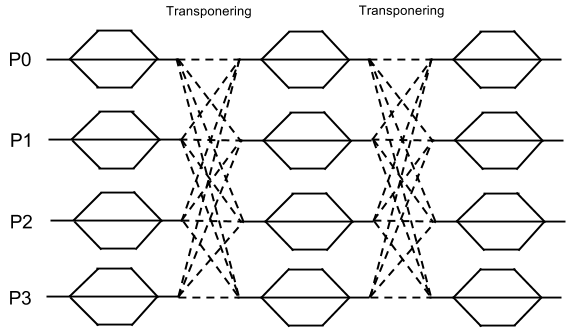
\includegraphics[width=10cm]{img/poisson_parallel.png}	
	\caption{Parallell profil av \emph{poisson\_parallel()} med MPI og OpenMP.}
	\label{fig:poisson-parallel}
	
\end{figure}
\label{section:poisson_parallel}
Siden dette er den desidert viktigste funksjonen i vårt program, krever den en litt grundigere gjennomgang. For å parallelisere den utdelte koden har vi delt opp den store globale matrisen $\ub{B}$, og tildelt hver prosess rader fra denne. Siden den utleverte \emph{fst}-metoden kun krever at elementene ligger etter hverandre i minnet, trenger ingen endringer å bli gjort her, og prosedyren kjøres på hver enkelt rad.\\
\\
For å transponere matrisen i en parallell kontekst, har vi fulgt veiledningen i \cite{fast-poisson}. Denne går ut på å utnytte \emph{MPI\_Alltoallv}-kallet til å få alle prosesser til å sende og motta data fra hverandre. For å få til dette må man lage sendebuffere med tilhørende størrelses- og forskyvningsvektorer.\\
\\
For å paralellisere med OpenMP, har vi slått sammen så mange løkker som mulig og dekorert disse med \emph{\#pragma omp parallel for}. I tillegg til dette, må vi utvide lagringsplassen til det midlertidige \emph{fst}-bufferet $z$, slik at hver tråd får sitt eget buffer. Dette er gjort ved hjelp av OpenMP-kallene \emph{omp\_get\_max\_threads()} og \emph{omp\_get\_thread\_num()}.\\
\\
Hybrid-løsningen med både MPI og OpenMP, har totalt tre fork/joins og to alle-til-alle kommunikasjonsbolker. Profilen er vist i figur \ref{fig:poisson-parallel}. 

\section{Tester og resultater}

\paragraph{Hardware}
Alle våre tester er kjørt på Kongull-clusteret. Dette clusteret benytter seg av CentOS 5.3 med Rocks på HP-servere, og består av 93 beregningsnoder. Hver node har 2x6-kjerner 2.4 GHz AMD Opteron 2431 (Istanbul)-prosessorer og 24 GiB minne. For flere detaljer, se \cite{kongull-hardware}.  

\paragraph{Kompilering og biblioteker}
Ved kompilering, hadde vi lastet inn modulene \emph{intelcomp/11.1.059}, \emph{cmake/2.8.7} og \emph{openmpi/1.4.3-intel}. CMake ble konfigurert med \emph{CMAKE\_BUILD\_TYPE=1}, \emph{ENABLE\_OPENMP=1} og \emph{ENABLE\_MPI=1}, og gitt environmentvariablene \emph{CC=icc}, \emph{CXX=icpc} og \emph{FC=ifort}. Programmene ble da kompilert med Intel-kompilatoren for det korresponderende språket. Programmene ble kompilert med optimaliseringsflagg \emph{O3}. Alle testene vi kjørte benyttet seg av disse instillingene, og for å regulere bruken av MPI og OpenMP brukte vi løsningen beskrevet i paragrafen om \emph{Flagg for MPI og OpenMP} i seksjon \ref{section:programkomponenter}.

\paragraph{Tidtakning}
Alle våre tidsmålinger er resulat av følgende prosess: Programmet ble kjørt ti ganger, de to minste og de to største verdiene ble forkastet, og gjennomsnittet av de seks resterende tidene ble brukt.


\subsection{Kjøretid med forskellige p*t = 36}
\label{subsection:runtime}
Denne testen ble gjennomført for noen kombinasjoner som gir \emph{p} * \emph{t} = 36. Resultatet er vist i tabell \ref{p/t-table}.

\begin{table}
\begin{center}
	
	\begin{tabular}{c | c | c}
	\hline \hline 
	Antall prosesser      &    Antall tråder     &    Kjøretid (i sekunder) 	    \\ \hline	
	12		      &		1	     &	  32.690540       		    \\ \hline
	6		      &         2	     &    32.975599       		    \\ \hline
	4		      &         3	     &    33.223129	    		    \\ \hline
	3   		      &		2	     &    33.633001	    		    \\ \hline
	2		      &         6	     &    34.279941	    		    \\ \hline
	1		      &		12	     &    35.741616	    		    \\ \hline
	
	\end{tabular}
\end{center}
\caption{Kjøretider gitt forskjellige kompinasjoner av \emph{p} og \emph{t}.}
\label{p/t-table}
\end{table}

Som tabell \ref{p/t-table} viser, er det faktisk negativt å bruke en hybrid-løsning. Vi ser at kjøretiden blir litt større jo flere tråder vi bruker. Grunnen er at det koster å opprette og samle tråder. Så i dette tilfellet lønner det seg dermed å kjøre programmene med kun en tråd. 
Testene som følger denne vil dermed kun bruke en tråd og heller variere antall prosesser. 

\subsection{Verifisering av korrekthet - Konvergenstester}
\begin{figure}[t]
	\centering
	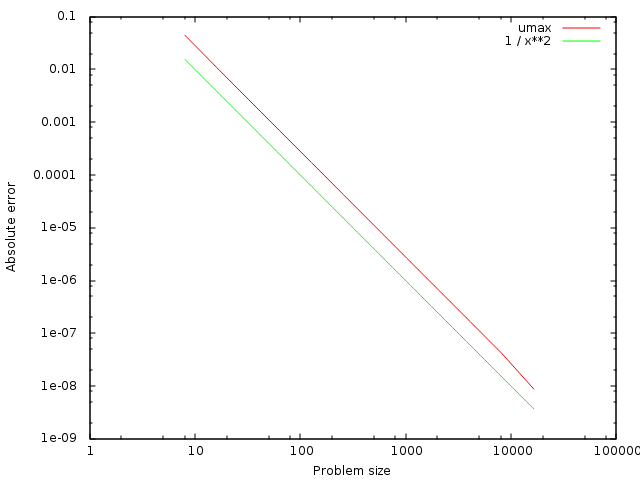
\includegraphics[width=8cm]{img/convergence.png}	
	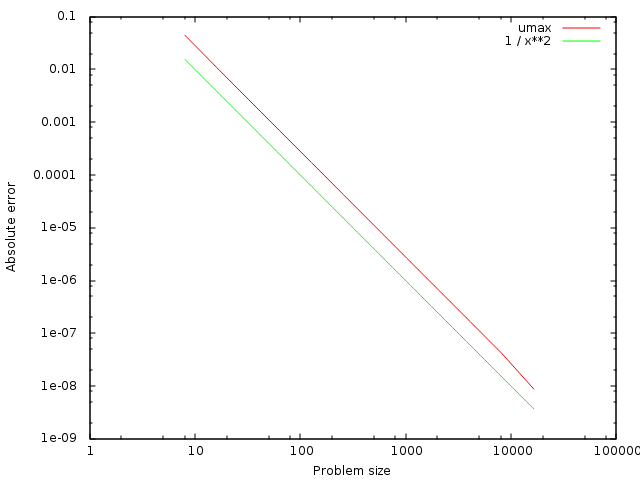
\includegraphics[width=8cm]{img/convergence.png}	
	\caption{Konvergenstester med ($p=12$, $t=3$) og ($p=36$, $t=1$).}
	\label{fig:convergence}
	
\end{figure}

Samtidig med testingen utført i seksjon \ref{subsection:runtime}, verifiserte vi også at de samme $p$- og $t$-verdier gav riktige resultater. Vi kjørte \emph{convergence} på intervallet n=8 til n=16384 og plottet resultatene opp mot ${1 \over x^2}$ i et log-log-plot. Dersom linjen som viser maksimal feil er parallell med referansefunksjonen, kan vi konkludere med at løsningen konvergerer og er følgelig korrekt. Samtlige kjøringer med ulike $p$- og $t$-verdier konvergerte. Kjøring med ($p=12$, $t=3$) og ($p=36$, $t=1$) er vist i figur \ref{fig:convergence}.

\subsection{Speedup og effektivitet}

Speedup sier noe om hvilken faktor vi ønsker at kjøretiden skal bli redusert med. Speedup er definert i ligning \ref{speedup}, der $S_p$ er speedupen, $T_1$ er kjøretiden på en prosess og $T_p$ er kjøretiden på P prosesser. Det vi ser i ligning \ref{speedup} er det vi kaller perfekt speedup, som vil si at kjøretiden reduseres med en faktor proporsjonal med antall prosesser. Gitt perfekt speedup ser vi da at $T_p$ må være definert som kjøretiden på en prosess, $T_1$, dividert med antall prosesser P som vist i ligning \ref{t_p}.  

\begin{equation}
	\label{speedup}
	S_{p} = {T_{1} \over T_{p}} = P
\end{equation} 

\begin{equation}
	\label{t_p}
	T_{p} = {T_{1} \over P}
\end{equation}

Det er derimot ikke gratis å sende data over nettverk. Dermed må en forvente at $S_p$ $<$ P. Overføringstiden, $T^{comm}$, avhenger av hva slags \emph{cluster} programmet kjøres på (overføringshastighet og invers båndbredde) og ikke minst hvor mye data som overføres. Generelt gjelder ligning \ref{t_comm}, der $\kappa$ er overføringshastigheten, $\gamma$ er den inverse båndbredden og b antall bytes som overføres.

\begin{equation}
	\label{t_comm}
	T^{comm}(b) = \kappa + \gamma b
\end{equation} 

Hvis vi antar perfekt speedup og siden vi gjør to transponeringer, kan en ved hjelp av ligning (\ref{speedup})-(\ref{t_comm}) utlede den teoretiske speedupen for vårt problem er (overføringshastigheten og invers båndbredde er gitt på forhånd):

\begin{equation}
	\label{theo_s}
	S_{p}^{theoretical} = {P \over 1 + 2(\kappa + \gamma 8N^{2})}, \text{der $\kappa$ = $10^{-6}$, $\gamma$ = $10^{-10}$}
\end{equation}

\begin{equation}
	\label{eff}
	\eta_{p} = {S_{p} \over P} 
\end{equation}

I ligning \ref{theo_s} har vi også antatt at prosessene sender data til seg selv. Selv om noen av elementene ikke vil bli sendt over nettverk, vil antall bytes i data være avhengig av problemstørrelsen. Dermed har vi sett bort ifra de små datamengdene som blir igjen hos hver prosess. Den teoretiske speedupen er et mer realistisk mål å oppnå, da den tar med overheaded ved dataoverføring. \\ 

Effektiviteten er definert som speedup dividert med antall prosesser, vist i ligning \ref{eff}. \\ 

Figur \ref{fig:speedup} og figur \ref{fig:eff} viser speedupen og effektiviteten for forskjellige antall prosesser for dataene i tabell bla og tabell bla i appendix bla1. I figurene har vi også tatt med teoretisk speedup og effektivitet for N = 16384. I figur \ref{fig:eff} har vi også fjernet de to laveste problemstørrelsene vi kjørte målingene på. Vi synes de bare var i veien i figuren og at dataene vist er mer en nok for å trekke ut nødvendig informasjon. \\

Som vi ser ut ifra figur \ref{fig:p96}, vil det ved store problemstørrelser bli en tilnærmet firedobling i tidsbruk. Dette er et absolutt forventet resultat. Ved små problemstørrelser ser vi litt mer varierte resultat. Grunnen er at overheaded ved sending av informasjon blir for stort sett mot problemstørrelsen. 

Vi ser også at speedupen blir bedre jo større problemstørrelse vi har. Dette ser en utifra figur \ref{fig:speedup}.

\begin{figure}[t]
	\centering
	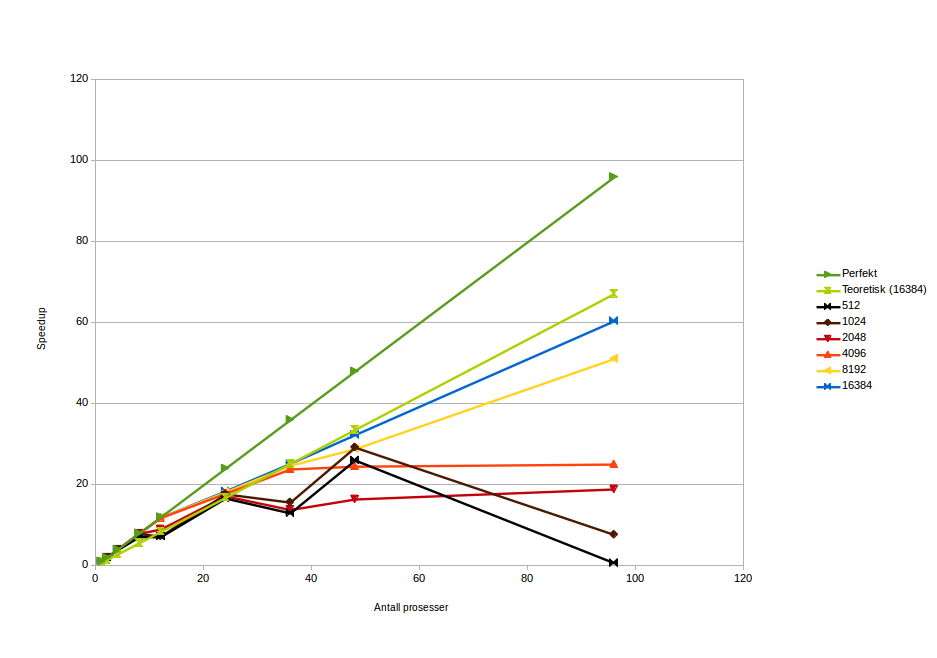
\includegraphics[width=12cm]{img/speedup.png}
	\caption{Speedup}
	\label{fig:speedup}
		
\end{figure}

\begin{figure}[t]
	\centering
	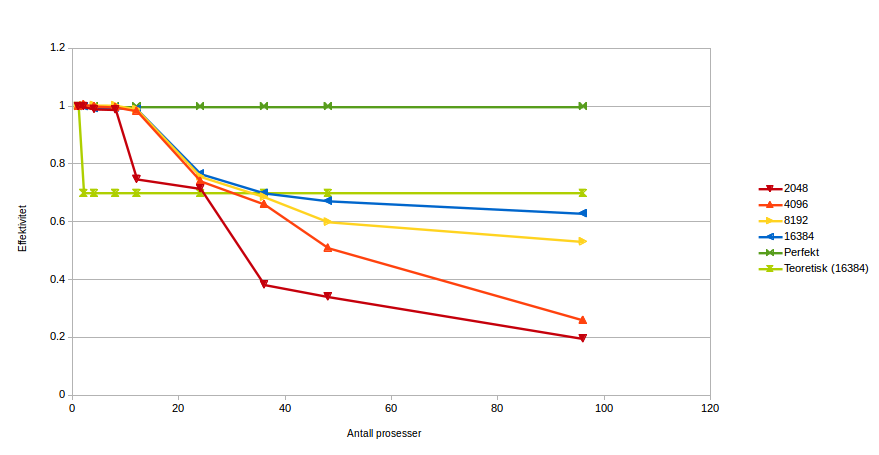
\includegraphics[width=12cm]{img/efficiency.png}
	\caption{Effektivitet}		
	\label{fig:eff}
\end{figure}

\begin{figure}[t]
	\centering
	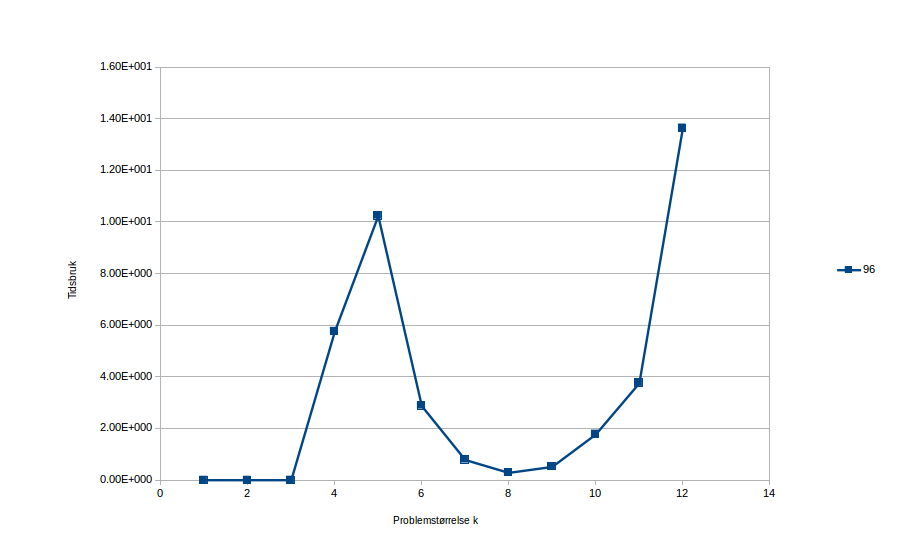
\includegraphics[width=12cm]{img/time_p_96.png}
	\caption{Tidsbruk ved 96 prosesser ved forskjellige k (n = $2^{k}$)}		
	\label{fig:p96}
\end{figure}


\section{Diskusjon og konklusjon}


\subsection{Å gå bort fra $f=1$}
\begin{figure}[h]
	\centering
	\lstinputlisting[frame=single, numbers=left]{code/local_f.c}
	\caption{Gå fra $f=1$ til en hvilken som helst funksjon $f(x, y)$.}
	\label{fig:local_f}
\end{figure}
For å håndtere en hvilken som helst todimensjonal funksjon $f(x, y)$, var det eneste som måtte gjøres å fylle ut $\ub{B}$ med verdier fra denne funksjonen. Her måtte vi bruke de lokale indeksene for å mappe $x$- og $y$-verdier og multiplisere funksjonsverdiene inn i matrisen. For å få dette til å kjøre i parallell måtte vi gjøre noen små justeringer når det gjaldt mapping fra lokale indekser til $x$- og $y$-verdier. Hver prossess lagrer kun sine egne rader, og en indeks til en rad i sin delvise (lokale) matrise vil mappe til en indeks i den fullstendige (globale) matrisen. Vi måtte derfor plusse på et offset på rad-indeksen når vi regnet ut verdien av $y$. Å gå fra $f=1$ til $f(x, y)$ fjerner med andre ord ikke noe parallelt potensiale, siden løkken som legger inn verdier i $\ub{B}$ ikke får noen avhengigheter som gjør at den ikke kan paralleliseres.

\subsection{Ikke-homogene Dirichlet grensebetingelser}
\begin{figure}[h]
	\centering
	\lstinputlisting[frame=single, numbers=left]{code/non_homogenous_dirichlet.c}
	\caption{Pseudokode for å addere grensebetingelsene inn i ligningssystemet.}
	\label{fig:non_homogenous_dirichlet}
\end{figure}
Dersom $u \neq 0$ i $\partial\Omega$, får vi ikke-homogene Dirichlet grensebetingelser. På generelt basis må man addere grensebetingelse inn i løsningsvektoren $\ub{b}$, eller i vårt tilfelle matrisen $\ub{B}$. Alle punkter i rutenettet som er nær en kant, må addere inn grensebetingelsene, det vil si verdiene til $u$ i $\partial\Omega$. En grov skisse av dette finner du i figur \ref{fig:non_homogenous_dirichlet}. \\
\\
Siden vi benytter oss av \emph{Fast Sine Transform} i denne oppgaven, må vi også være observante på hvordan grenseverdiene er definert. Dersom de er definert som Dirichlet grensebetingelser (vi kjenner verdien av $u(x, y)$ hvor $(x, y)\ \epsilon\ \partial\Omega$) vil sinustransformen fremdeles fungere.\\

\subsection{Piossonproblemet der $\Omega = (0, L_x) \times (0, L_y)$}
For å ta høyde for domener som ikke er definert som et enhetskvadrat, er det flere ting som må gjøres. For det første må vi gjøre om $h$ til $h_x = {L_x \over n}$ og $h_y = {L_y \over n}$. Mappingen på linjene 2 og 3 i figur \ref{fig:local_f} måtte da justeres til å ta høyde for disse ved å multiplisere hver indeks med korresponderende $h$-verdi i stedet for å dividere på $n$. I tillegg vil vi ikke lenger kunne multiplisere inn $h^2$ i steg 1, så steg 2 må modifiseres til å håndtere dette.\\
\\
Det er viktig å understreke at endring av $\Omega$ kun endrer på det fysiske domenet, ikke det logiske. Det er derfor ingen endringer som må gjøres i FST-algoritmen eller i utregning av diagonalen. Siden vi benytter oss av en direkte metode, vil vi ikke lide av ytelsestap, noe iterative metoder ofte gjør.
\subsection{Forslag til forbedringer}

\begin{thebibliography}{9}

\bibitem{ps6}
	Rønquist, Einar M. (2014),
	\emph{TMA4280 - Problem set 6}

\bibitem{poisson}
	Rønquist, Einar M. (2014),
	\emph{The Poisson problem as a model problem}.
	Revidert av Kvarving, Arne M. (2014)

\bibitem{poisson-fdm}
	Rønquist, Einar M. (2014),
	\emph{The Poisson problem: finite difference techniques}.
	Revidert av Kvarving, Arne M. (2014)

\bibitem{rdw}
	\emph{Reaction-Diffusion workshop} (2014),\\
	Tilgjengelig fra: http://n-e-r-v-o-u-s.com/education/simulation/ethworkshop.php
	(Hentet: 31.03.2014)

\bibitem{buffalo}
	\emph{Chapter 6, Partial Differential Equations, Lecture 2} (2004),\\
	Tilgjengelig fra: http://www.physics.buffalo.edu/phy410-505-2004/Chapter6/ch6-lec2.pdf
	(Hentet 01.04.2014)
\end{thebibliography}

\end{document}
